%Submission Contents
%Declaration of Conflict


\section{Company Profile}
\label{intro}

PowerCore Engineering is an established and recognized leader in Ontario providing services and solutions in power and energy management systems. Located in London, PowerCore Engineering has over 15 years of experience and has provided services to over 200 customers. Since 2008 PowerCore has expanded internationally delivering services and products to China, Brazil, Mexico and the United States.\\

PowerCore Engineering prides itself in high level of in-house knowledge and expertise in power system engineering, engineered drive systems, power monitoring  energy management solutions, SCADA systems and BMS systems. \\

PowerCore is a certified system integrator for Schneider ION Power Monitoring and Energy Management product line. PowerCore Engineering is also an elite system integrator for Yaskawa Variable Frequency Drives, ASCO Transfer switches, GE Products, Delta V, Alerton, PowerIT Spara demand control products, Eaton Power Monitoring and Energy Management products. Our expertise is however not limited to these types of product, but reaches far into all aspects of power system design/management, BMS and SCADA systems.\\

We deliver services to commercial, institutional and industrial establishments and have the capacity to provide solutions ranging from a limited scope to very challenging projects.\\

PowerCore Engineering excels in energy management solutions applying our knowledge and expertise at each and every phase of the project.  We have the capability to design/build a power monitoring system, install and configure the required hardware, configure the necessary communication and networking channels, develop customized interface, prepare periodic reporting structure and provide extensive post-project support. \\

PowerCore has catered to many specific requirements for institutional and industrial applications with user specific designs, such as:
\begin{itemize}
	\item Web Browser and workstation based Energy Management Dashboard in a University setting to keep various access level clients around campus informed about user-specific electric info such as system loading, energy consumption, WAGES costing e.t.c. utilizing mutli-platform devices.
	\item Internally developed BACnet to Modbus HTML 5 based bi-directional protocol translator to cost effectively poll data from Modbus devices (ie. Power Meters and VFDs) into BACnet based BMS systems (ie. Alerton and Delta V) without the need for dedicated hardware translators. 
	\item Web Browser and MS Excel based custom reports and demand and Energy charges allocation for individual and aggregated meters.
	\item Creating and maintaining a MS SQL Server based power monitoring database for real time access by third party applications via \textbf{OPC} and \textbf{DDE}.
	\item Modernizing systems to utilize the latest variable frequency drives and lighting technology while taking advantage of Save On Energy incentives.
\end{itemize}

We believe in control and reduction of energy consumption and the ability to control demand by utilizing the latest technologies. Our mission is to empower customers to take control of their peak energy usage allowing them to operate with greater efficiency while reducing energy costs by monitoring, analyzing, and controlling their system.\\


\noindent For more info please refer to our page at: \url{http://www.powercore.ca}\\

\pagebreak

\section{Expertise and Technical Qualifications}
\label{ETQ}

\subsection{Individual Expertise}
\label{ETQ:IndExp}

Please review PowerCore Engineering's Employee profiles in the following pages.  The Employees listed in this section will be assigned to perform the requested work.    

\includepdf[pages=-]{PowercoreEngineeringEmployeeCVs.pdf}

\subsection{PowerCore Engineering Expertise}
\label{ETQ:PCEExp}

\subsubsection{Energy Management}
\label{ETQ:PCEExp:EM}

PowerCore engineering is an authorized Schneider Electric 
\includegraphics[height=0.2in]{../Images/ecoxpert-logo.png} partner (one of four in Ontario) for Power Monitoring and Energy Management Solutions.\\

As such, we have to be intimately familiar with Ontario’s and the IESO Electricity billing structure ( i.e. kWh Energy usage billing and the kW Peak Demand billing), as well as Global Adjustment Class A and B billing structure.\\
 
We have implemented numerous energy reports based on Powerlogic - ION power monitoring system, reflecting Ontario specific billing structure (On-Mid-Off rates, HOEP pricing, etc.) for industrial/commercial and institutional customers.\\

We have also developed a customized Energy Billing Verification system application (ESSO IOL), to reconcile Daily \& Monthly billing, reflecting IESO data and internal power monitoring system data, as well as several site-specific cost allocation energy reports to determine cost-per-unit (industrial) of cost-per-occupant (institutional).\\

PowerCore engineering is also an exclusive Ontario partner with two significant players in the Electrical Demand management field:
\begin{itemize}
	\item NRG-ECS (Energy Curtailment Specialists) - One of three official aggregators with IESO for new capacity based Demand Response Program ( former DR3 program).  \textbf{PowerCore is an agent and integrator for ECS.}
	\item Spara-PowerIt  Demand control systems providing automated peak demand control system that can be tailored to customer specific needs: Monthly peak demand reduction, Fulfillment of the Demand Response obligations or Global Adjustment CP5 event management (for GA class A customers) .  \textbf{PowerCore is an agent and integrator for Spara.}
\end{itemize}

\pagebreak

\subsubsection{Power Monitoring/Energy Management Systems/Building Management Systems}
\label{ETQ:PCEExp:PM}

\noindent \textbf{Description:}\\
	
PowerCore Engineering has serviced and installed various management systems in a number of facilities.  These systems enable full overview and insight into existing and historical energy consumption. PowerCore has developed and implemented solution that allow this information to be accessed anywhere and at any time.\\ 

PowerCore Engineering is one of four officially authorized Schneider 
\includegraphics[height=0.2in]{../Images/ecoxpert-logo.png} partners in Ontario for Powerlogic-ION Power Monitoring and Energy Management Systems.\\

PowerCore Engineering can install new or utilize existing equipment to bring available data into an Energy Management System with a centralized approach to monitor and analyze Water, Air, Gas, Electricity, and Steam (W.A.G.E.S.) data.\\

PowerCore Engineering has provided customized solutions by: 
\begin{itemize}
	\item Utilizing existing communication-ready power meters and other devices
	\item Creating energy management dashboards and integrating W.A.G.E.S. data from multiple devices and platforms.
	\item Adding new monitors and devices in selected locations
	\item Integrating devices and statuses into various BMS platforms (Delta V, Alerton, and APOGEE)
	\item Providing customized energy and demand reports based on SQL database and/or MS Excel
	\item Implementing Web-based remote control and monitoring

\end{itemize}


PowerCore Engineering's team also possess the expertise to develop/implement Communication Protocol Conversion Applications in order to connect Legacy devices to new systems.\\ 

\vspace{10 mm}

\noindent \textbf{Experience:}

\begin{itemize}
	\item PowerCore Engineering has installed and serviced power monitoring systems in such facilities as The City of London, The University of Western Ontario, McMaster University, Wilfrid Laurier University, GlaxoSmithKline, Great Lakes Copper, Presstran, ESSO IOL, Electro-Motive Diesel, General Dynamics London, Liberty Freezers and a number of others.
	\item PowerCore Engineering is a certified integrator for Schneider and our team possess the skills and experience to work with any brand of Power Monitoring equipment and/or SCADA and BMS System.
\end{itemize}

\pagebreak

\subsubsection{Variable Frequency Drive (VFD) Applications and Lighting Retrofits}
\label{ETQ:PCEExp:VFD}


\noindent \textbf{Description:}\\
	

Whether it be for 
\includegraphics[height=0.1in]{../Images/SOE.png} incentives or system modernization, PowerCore Engineering has worked on a number of  VFD and lighting retrofit projects. In these projects PowerCore Engineering has provided the following: 
\begin{itemize}
	\item Designed both AC and DC motor test stations internationally. 
	\item Specified and provided Line/Load reactors for existing VFDs.
	\item Supplied, installed and programmed VFDs for single and multi drive systems.
	\item Implemented external control interfaces for various drive systems to external SCADA, BMS, and/or energy management systems.
	\item Engineered control and interface drawings for new builds.
	\item Reverse Engineered control and interface drawings for existing equipment without documentation.
	\item Liaison to local utilities to take advantage of the 
\includegraphics[height=0.1in]{../Images/SOE.png} incentives (Prescriptive and Engineered) for Lighting, VFD and motor upgrades.
	\item PowerCore Engineering utilizes Lande Associates for photometric evaluation to determine fixture spacing and luminosity specifications.
\end{itemize}

\vspace{10 mm}
\noindent \textbf{Experience:}	

\begin{itemize}
	\item PowerCore Engineering has provided VFD engineering, installation, integration and/or troubleshooting for the The Sleeman Center, AEP Canada, City of London, IPEX, Cementation, Natra, Electro-Motive Diesel, Goldcrop and others.
	\item PowerCore Engineering has supplied and managed installation of CFL lighting retrofit project and applied for Ontario save on rebates for General Dynamics Land Systems.

\end{itemize}

\pagebreak

	
\subsubsection{Power/Control System Troubleshooting }
\label{ETQ:PCEExp:TS}


\noindent \textbf{Description:}\\
	

PowerCore Engineering has experience with troubleshooting legacy drives, motor starters, customized control system and specialized I/O breakdowns.\\

PowerCore has assisted with the following: 
\begin{itemize}
	\item On-site/Off-site troubleshooting and repair of industrial and commercial electrical and electronic equipment
	\item Reverse engineering (re-constructed system drawings and operation manuals)
	\item Sourced outdated and rare equipment
	\item Replaced obsolete parts with up-to-date equivalents
	\item Re-design, supplied and installed unrepairable components and systems
\end{itemize}

\vspace{10 mm}
\noindent \textbf{Experience:}	

\begin{itemize}
	\item PowerCore Engineering has serviced and supports Controls/Drives Systems at Lambton Conveyor, AEP Canada and IPEX.  	
	\item PowerCore has also performed troubleshooting and recommissioning of Harvest Power and London District Energy's multi generator systems.
\end{itemize}

\pagebreak

\subsubsection{Portable Power Monitoring \& Power Quality Analysis}
\label{ETQ:PCEExp:PowM}


\noindent \textbf{Description:}\\
	

PowerCore Engineering has provided a portable power monitor where a power monitoring system is absent in order to provide on-the-spot power measurements to evaluate the following:
\begin{itemize}
	\item Load Flow
	\item Power Factor
	\item Excessive Harmonic Distortion
	\item Sub Cycle Transients
	\item Voltage Flicker
	\item Voltage Fluctuation
	\item Neutral Cable Overheating
	\item Ground Loops/Grounding Problems
\end{itemize}

Our Portable Power Monitoring Package based on PML ION 7500 meter provides all the necessary information within moments. The power monitors are typically installed in customer specified locations for a period of 1-7 days, but other arrangements are possible. \\

In order to mitigate power quality issues, PowerCore Engineering has provided such customized solutions as:
\begin{itemize}
	\item Fixed PF Correction Capacitor Banks
	\item Switched-in Capacitor Banks
	\item Harmonic Filters
	\item Voltage Regulators
	\item K-rated Transformers
	\item Transient Voltage Surge Suppressor (TVSS)
\end{itemize}


\vspace{10 mm}
\noindent \textbf{Experience:}

\begin{itemize}
	\item PowerCore has supplied and installed temporary power monitors in a number of locations.  Such locations include site for the city of London, Black Fly, Sealed Air, Electro-Motive Diesel, Formosa Springs Brewery, Great Lakes Copper and General Dynamics Land Systems.
	\item PowerCore Engineering has designed site specific condition filters for Panabrasive Inc, GM CAMI Assembly and Atlas Copco.
	\item PowerCore has installed and/or retrofitted power factor correction capacitor banks for a number of site such as The city of London, Great Lakes Copper, The Original Cakerie, Fischer Canada and a number of others. PowerCore has installed these capacitor banks in an economical manner with 2-3 year payback periods.
	\item PowerCore Engineering has specified and installed various TVSS for Wilfrid Laurier University and Great Lakes Copper in order to add reliable surge protection.
\end{itemize}

\pagebreak

\subsubsection{Power System Studies}
\label{ETQ:PCEExp:PSS}


\noindent \textbf{Description:}\\
	

PowerCore Engineering has extensive experience in engineering studies ranging from simple short circuit and protective coordination studies to complex power system modeling and system design. Some common power system studies are:
\begin{itemize}
	\item Short Circuit Evaluation and Protective Coordination Studies (typically required for all new installations, and advisable after substantial system alterations). This study is performed to evaluate and stipulate the settings for all protective devices including breakers, protective relays, fuses, motor protectors, etc. The results of which ensure optimum system protection in case of fault, i.e. the system branch is safely and selectively isolated before any damage to the system is sustained
	\item Load Flow and Voltage Stability Studies (voltage fluctuation projections, equipment loading assessments, etc.)
	\item Motor Starting Studies and Simulations (most often performed before large motor installations)
	\item Harmonic Analysis (PQ evaluation, capacitor impact forecast, harmonic filters design/specifications, etc.)
	\item Insulation Coordination Studies (HV and MV installations)
	\item Emergency Backup System Audits (power outage impact evaluations, backup system performance, generator/ATS sizing, power system tie-in considerations, etc.)
	\item Power System Design for Industrial and Commercial Facilities (drawings, engineering specifications, ESA submittals, contractor liaisons)
	\item Ground Grid Design (new and existing substations)
\end{itemize}

\vspace{10 mm}
\noindent \textbf{Experience:}

\begin{itemize}
	\item PowerCore provides Arc Flash Hazard Analysis for General Dynamics, Presstran, Meritor Suspension Systems Company (MSSC), The University of Western Ontario, Fanshawe College, Electro-Motive Diesel and a number of others. 
	\item Specifically for the City of London and Wilfrid Laurier University, PowerCore has annual contracts to analyze facilities with and without Arc Flash Analysis; Running full analysis on facilities that require analysis and updating those that are out of date. In many cases additional protective device coordination studies are typically conducted to maintain selectivity and reduce the arc flash hazard through means of circuit protection adjustments. 
	\item PowerCore has also provided load flow analysis and motors starting studies for companies like Enbridge Pipeline and Henry Company Canada in order to troubleshoot power quality issues, optimize transformer on-load tap changers and examine feasibility for new installations.
\end{itemize}

\pagebreak

\subsubsection{Mechanical Engineering}
\label{ETQ:PCEExp:Mech}
PowerCore Engineering utilizes Somers Environmental Products Inc. and their subcontractors in order to provide access to custom Air Handling Units, Unit Heaters, Fan Coils, Terminal Heating Units, Chilled Beams, Fans, Humidifiers, Boilers and Variable Air Volume Boxes. Somers, also based in London, has a long standing relationship with contractors in Kitchener for mechanical/sheet metal field services that will be utilized for this project.\\

\noindent For more info please refer to their web page at: \url{http://www.somersep.com/}\\

\pagebreak

\section{Consistency in Staffing}
\label{CS}

PowerCore Engineering will be utilizing the employees listed in the \hyperref[ETQ:IndExp]{Individual Experience} section to perform the requested services.  A lead employee will be assigned to this account when the project is awarded. The lead employee will draw on other team members to service the customer's needs.  In the event of an emergency call, the lead contact will be dispatched.  In the unlikely event where the project lead isn't available, a secondary contact will be dispatched.  The secondary contact will be elected internally based on past experience and knowledge of the system. 

\pagebreak

\section{Response Time and Availability}
\label{RTA}

PowerCore Engineering's office hours are from 8 am to 4:30 pm.  If an emergency arises outside of the office hours, over time rates will apply.  PowerCore Engineering's Office is located just off the 401, therefore the typical response time to an emergency call will be 1 hour and 20 minutes.  If emergency call is placed after hours, the response time may be extended to the 1 hour and 50 minutes for additional travel to the office to collect any tools.  Also, depending on the nature of the issue, PowerCore may be able to provide assistance remotely.  

\pagebreak

\section{Invoicing}
\label{Inv}

PowerCore Engineering utilizes Quickbase Customer Relationship Management software for accurate invoice processing and tracking.  This management software, in conjunction with PowerCore's internal practices for tracking employee time ensure that billing remains organized.  PowerCore Employees are responsible for filling out time-sheets daily and biweekly are required to submit their time for review.\\

Invoices are typically sent over email and include work order numbers and descriptions as reference for customers.  If Jobs are completed on a time and material structure, the R/T, O/T and material are all displayed as separate line items.  Invoice structure can be modified to fit customer needs, but PowerCore has been successful using the structure similar to the \hyperref[fig:Ir5000]{sample invoice} displayed in this section.\\

PowerCore also submits status reports when working on larger project that help keep the customer informed and to ensure there are no surprise costs when invoiced. Please see  \hyperref[fig:Page1OfProgressReport]{Page 1} and \hyperref[fig:Page2OfProgressReport]{Page 2} of the example Progress Summary in the following section.\\

%\includepdf[pages=-]{Ir-5000.pdf}

\begin{figure}
		
		\begin{center}
		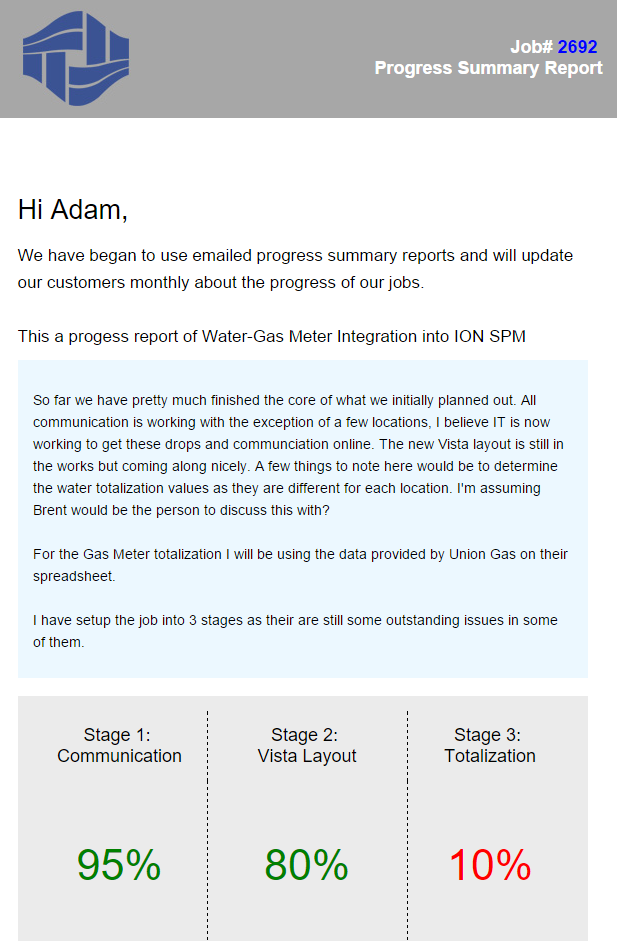
\includegraphics[width=5in, keepaspectratio=true]{../Images/ProgressReport1.PNG}
		\end{center}
	\caption{Page 1 Of Progress Report}
	\label{fig:Page1OfProgressReport}
\end{figure}



\begin{figure}
		
		\begin{center}
		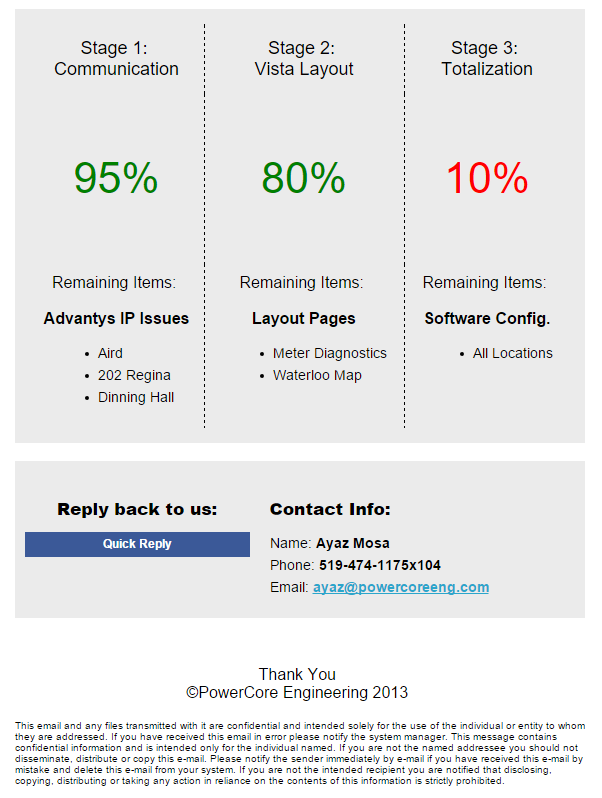
\includegraphics[width=5in, keepaspectratio=true]{../Images/ProgressReport2.PNG}
		\end{center}
	\caption{Page 2 Of Progress Report}
	\label{fig:Page2OfProgressReport}
\end{figure}



\begin{figure}
		
		\begin{center}
		\includegraphics[width=6in, keepaspectratio=true]{../Images/Ir-5000.png}
		\end{center}
	\caption{Sample Invoice}
	\label{fig:Ir5000}
\end{figure}

\pagebreak

\section{Previous Company Experience (CONFIDENTIAL)}
\label{PreExp}

A broad overview of PowerCore Engineering's relevant previous experience has been covered in the \hyperref[ETQ:PCEExp]{Expertise and Qualifications} section of this proposal.  In this section, PowerCore will present specifics on past projects illustrating past experiences with BAS, SCADA, power monitoring and complex controls systems.

\subsection{Wilfrid Laurier University - Waterloo, Ontario}
\label{PreExp:WLU}
	
	\begin{itemize}
		\item Installed, configured, and integrated over 40 power meters; tying in all power meters onto internal network
		\item Installed and configured power monitoring software, adding all power meters and custom aggregation calculations of various buildings. 
		\item Installed and maintained top-tier Energy Management software and tied into existing power monitoring software.
		\item Prepared OPC export tags of each essential meter measurement to be utilized by third party software applications
		\item Ran communication of all water and gas meters around campus as digital inputs and added them to existing power monitoring software.
		\item Maintain power monitoring database, computer system and provide continuing support.
		\item Rebuilt existing power monitoring web interface to incorporate a functional user friendly designed web enabled dashboard site (displayed over the next few pages). 
	\end{itemize}

\pagebreak

	\begin{center}
	\begin{figure}
			
\includegraphics[height=5in]{../Images/WLU1.png}
		\caption{Main Dashboard}
		\label{fig:MainDashboard}
	\end{figure}

	\end{center}


	\begin{center}
	\begin{figure}
			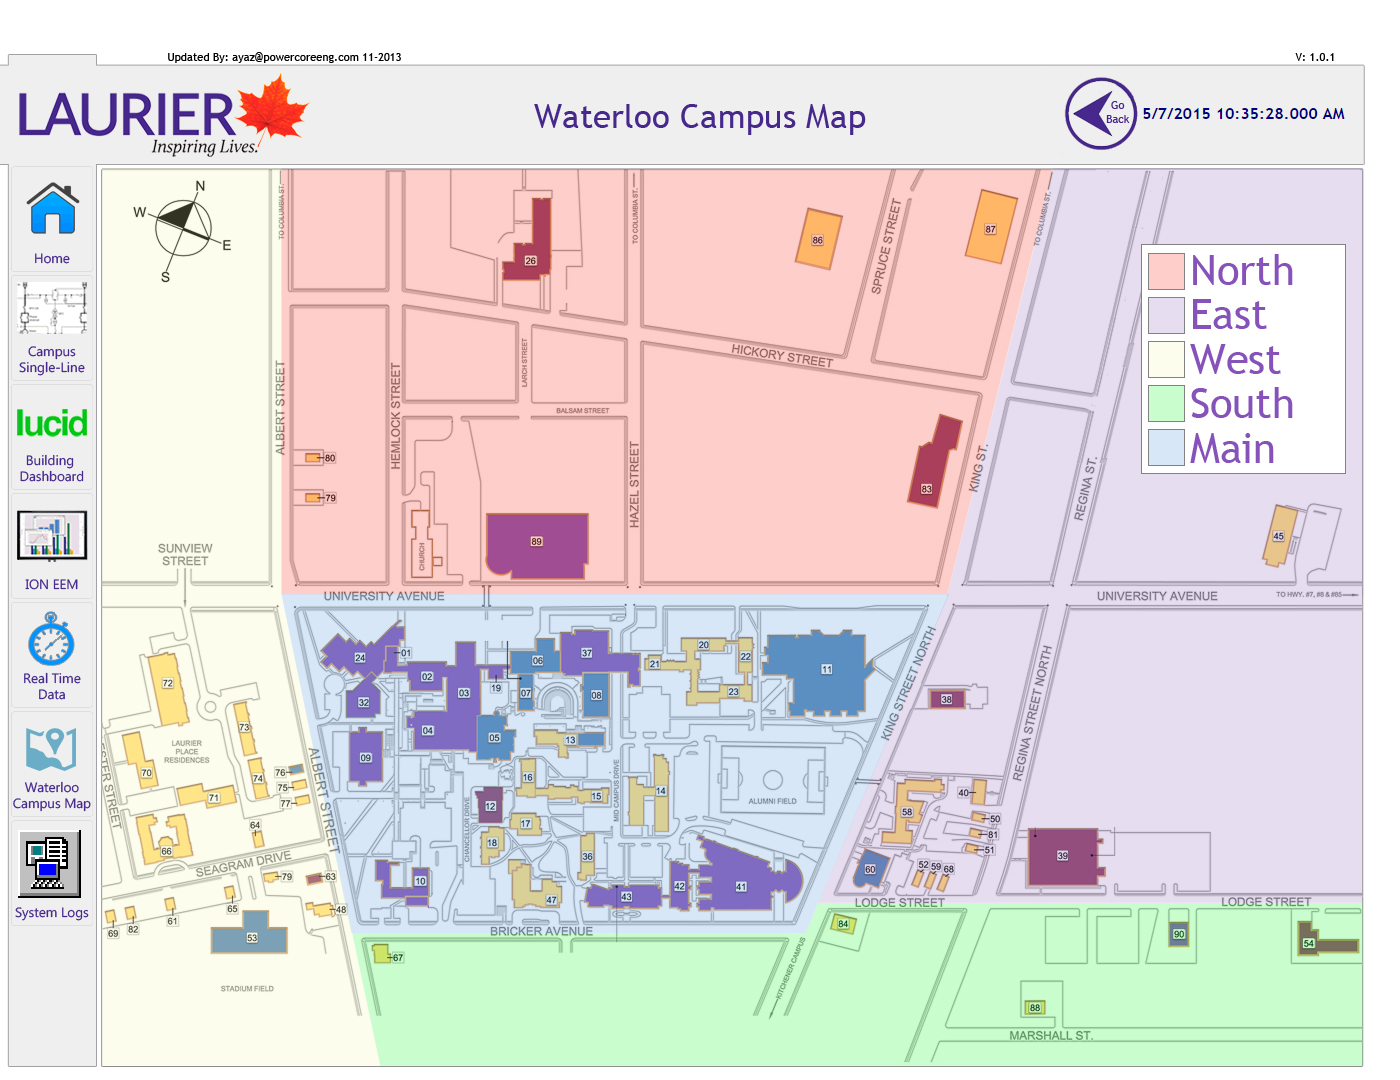
\includegraphics[height=5in]{../Images/WLU2.png}
		\caption{Full Campus Map}
		\label{fig:CampusMap}
	\end{figure}
	\end{center}


	\begin{center}
	\begin{figure}
			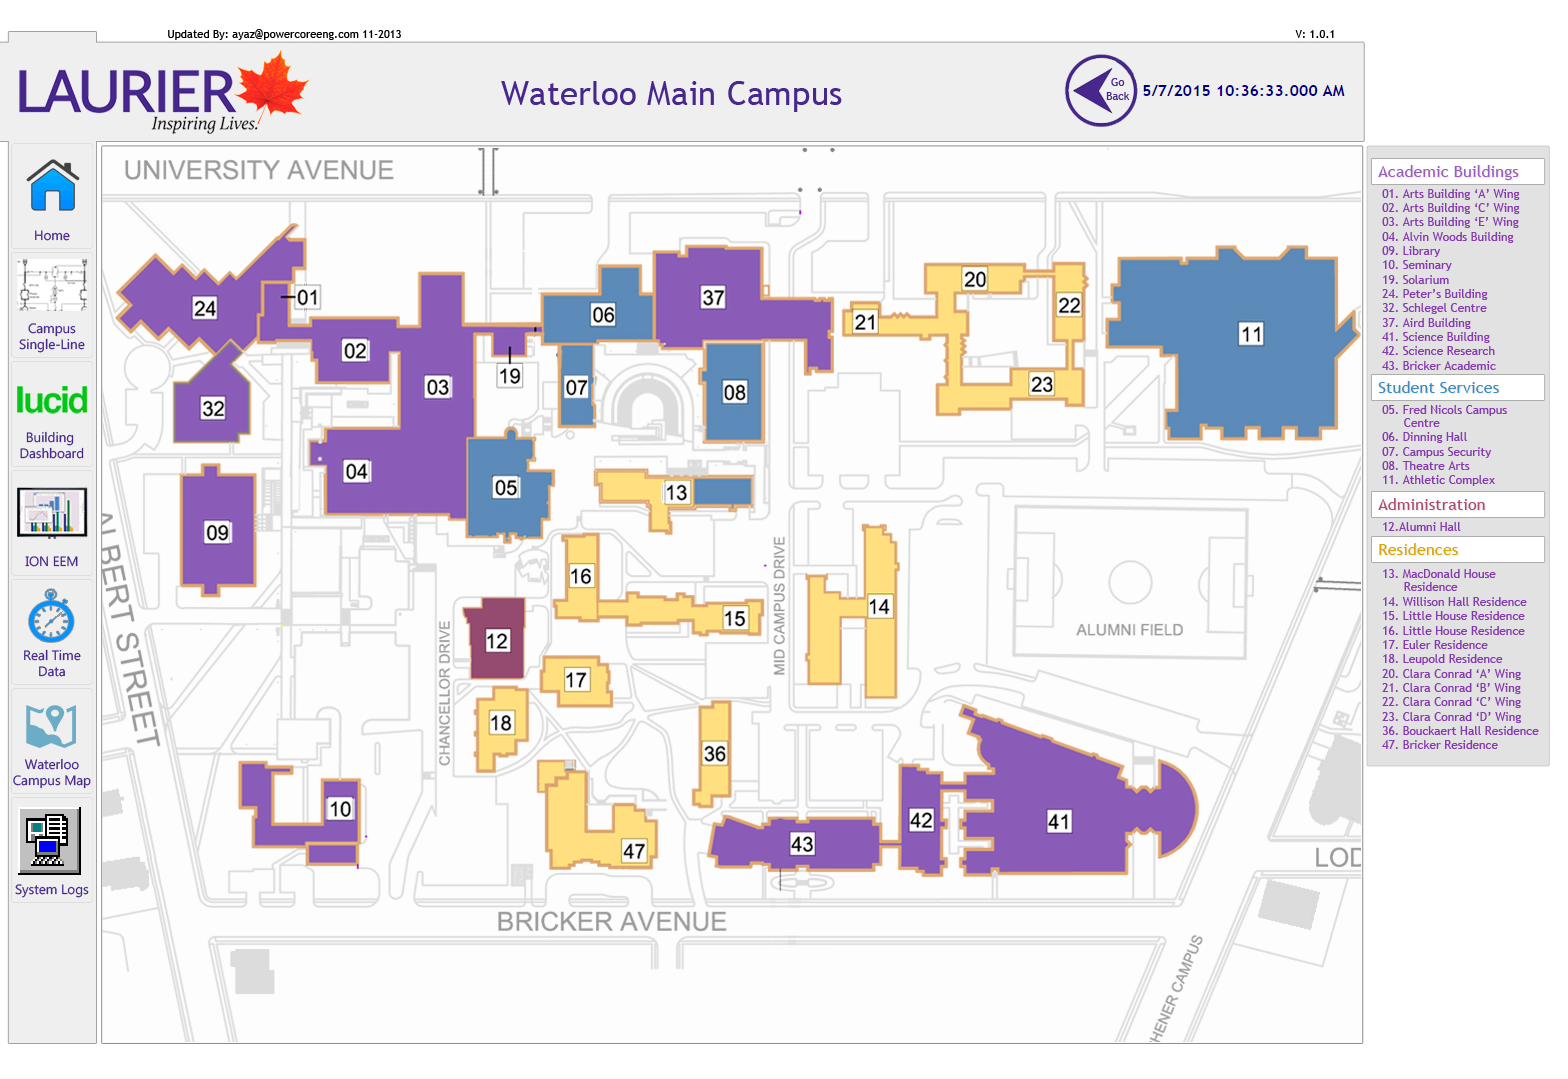
\includegraphics[height=5in]{../Images/WLU3.png}
		\caption{Main Campus Map}
		\label{fig:MainCampusMap}
	\end{figure}
	\end{center}


	\begin{center}
	\begin{figure}
			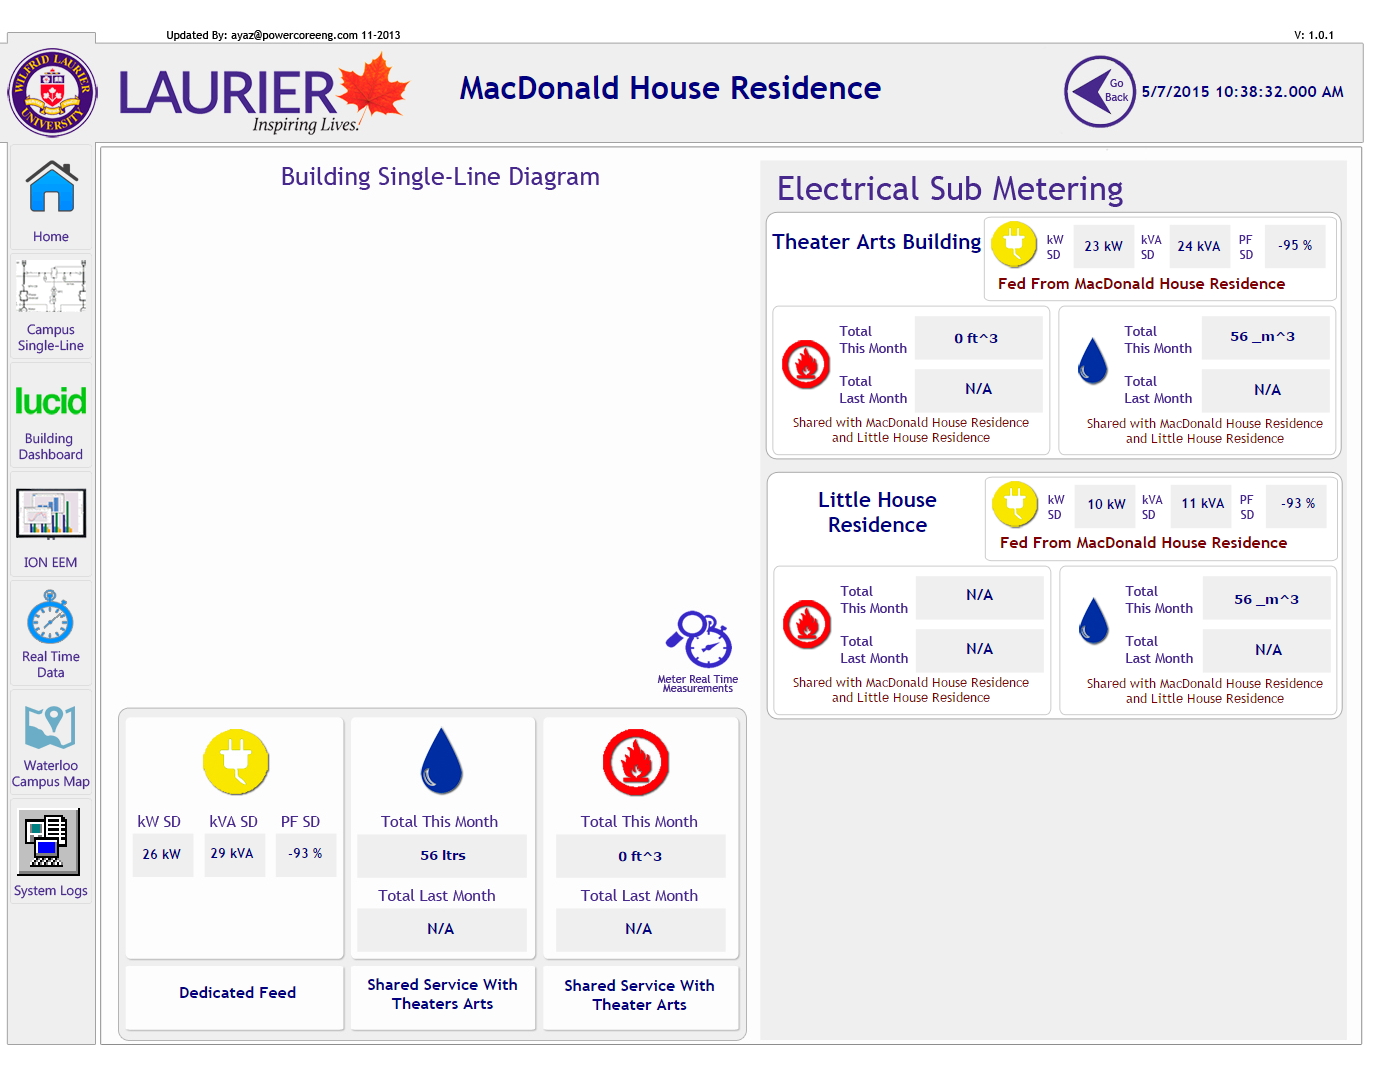
\includegraphics[height=5in]{../Images/WLU4.png}
		\caption{Residence Dashboard}
		\label{fig:ResidenceDashboard}
	\end{figure}
	\end{center}


	\begin{center}
	\begin{figure}
			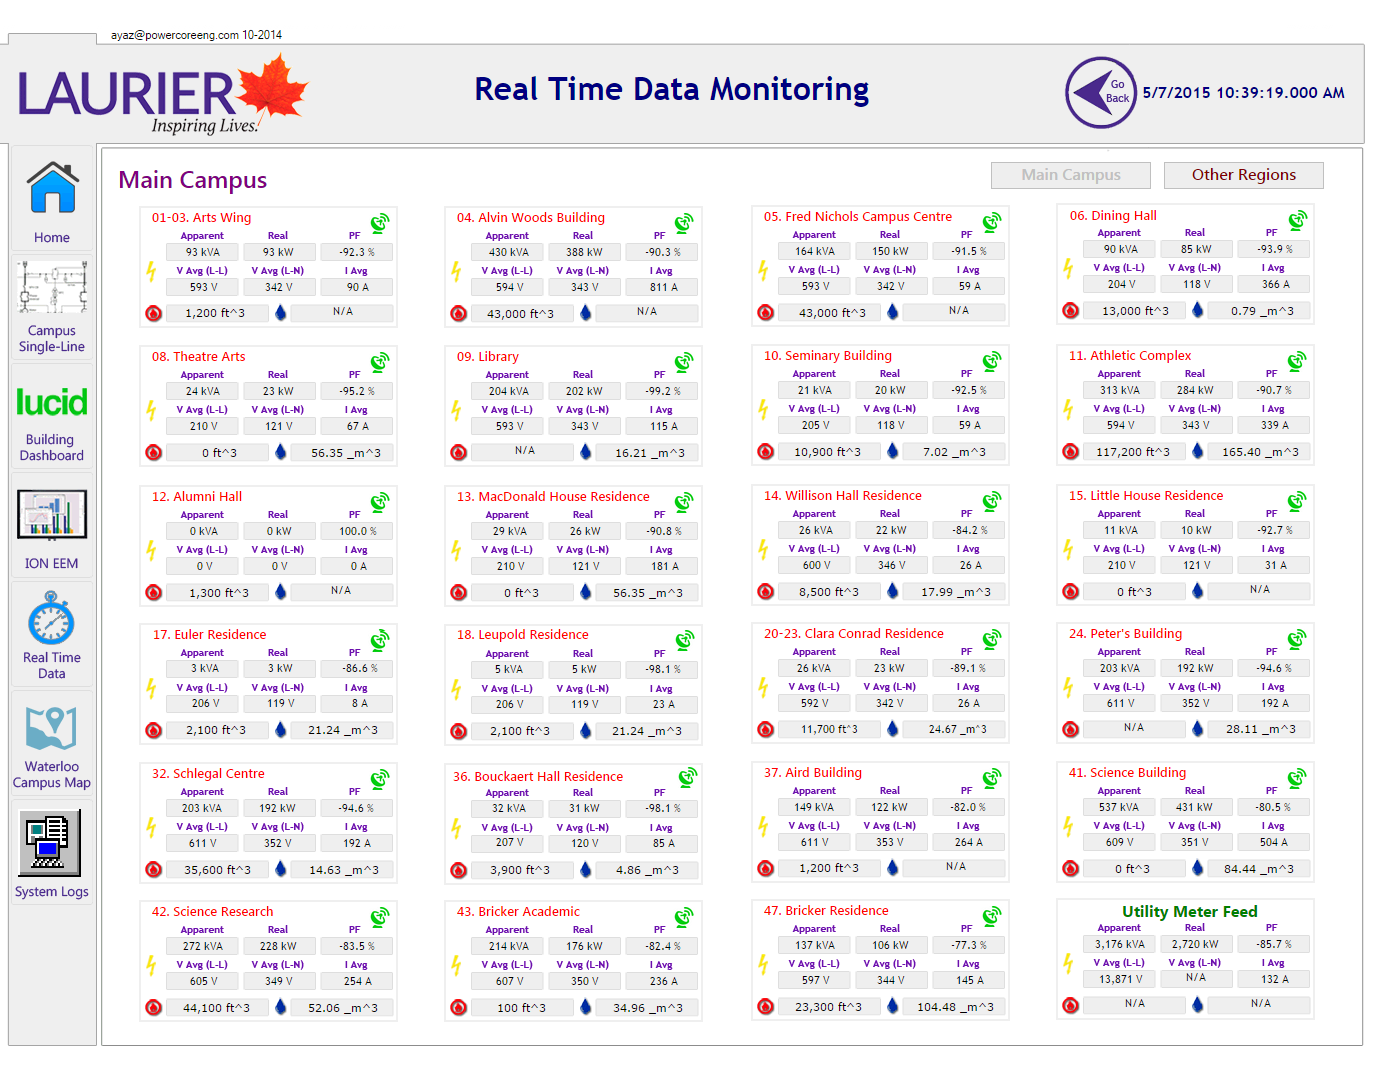
\includegraphics[height=5in]{../Images/WLU5.png}
		\caption{Real Time Data Monitoring}
		\label{fig:RealTimeDataMonitoring}
	\end{figure}
	\end{center}


	\begin{center}
	\begin{figure}
			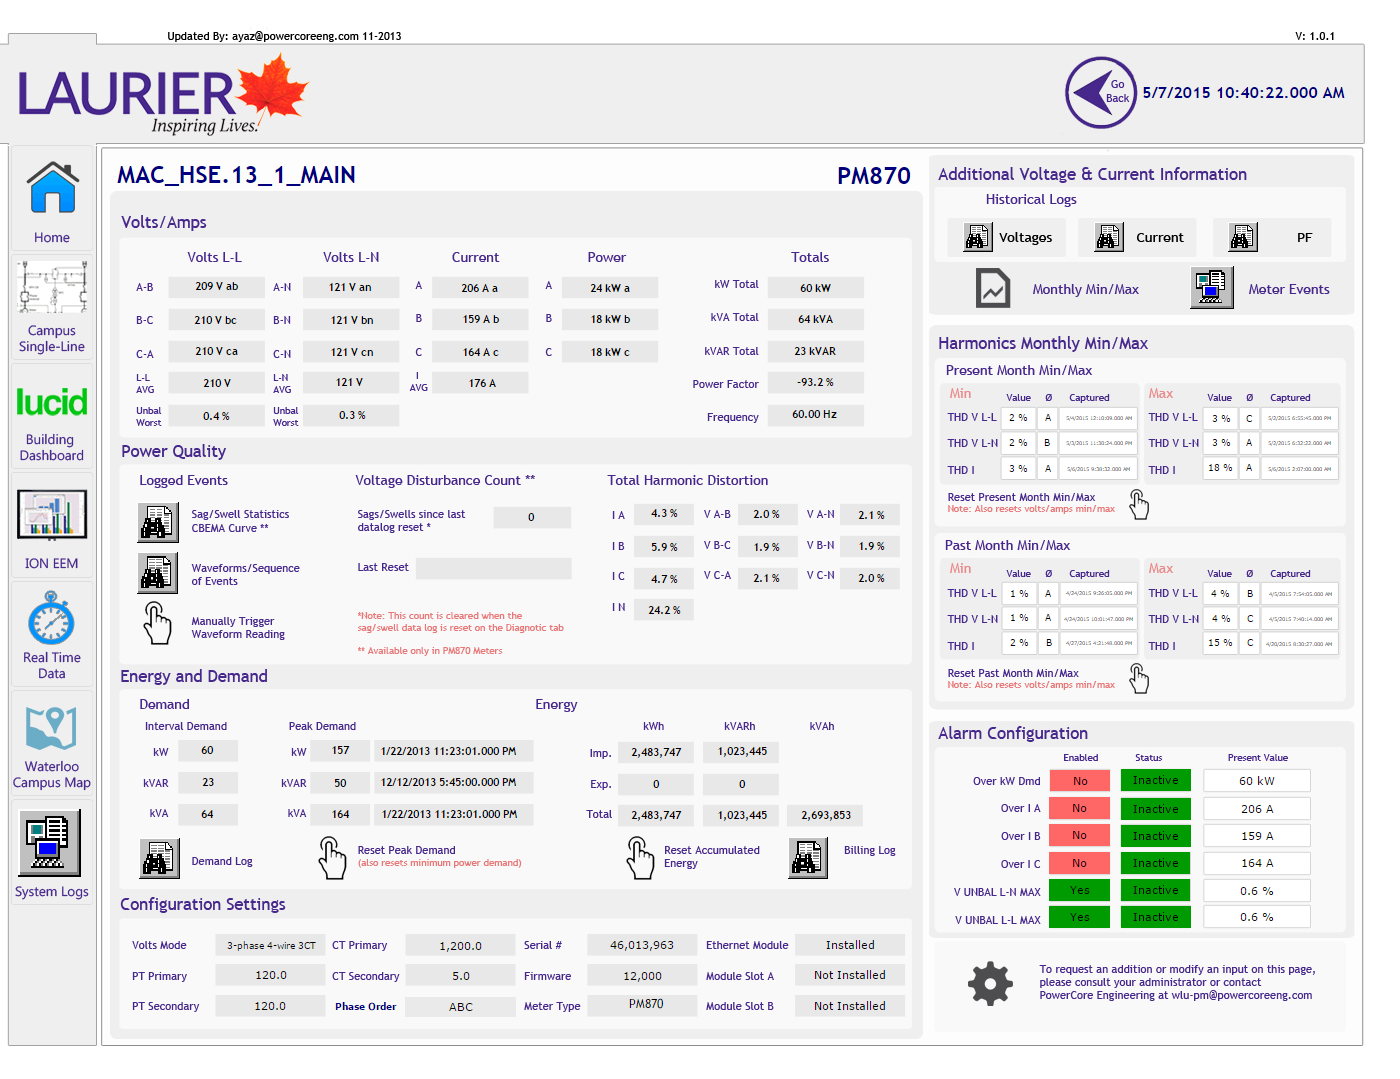
\includegraphics[height=5in]{../Images/WLU6.png}
		\caption{Individual Meter Dashboard}
		\label{fig:IndividualMeterDashboard}
	\end{figure}
	\end{center}

\pagebreak


\subsection{Electromotive Diesel/Caterpillar/Progress Rail - International}
\label{PreExp:TMTS}

\begin{itemize}
	\item Design-built multiple turnkey AC Traction Motor Test Station with 2,300V/150A AC VFD Power Supply (using 600HP LV VFD \& Step-up Trfm).
	\item Design-built multiple turnkey DC Traction Motor Test Station with 2,000V/100A DC \& 60V/1200A DC Power Supplies (using LV VFD,  Transformers \& rectifiers).
	\item Each system utilized MV Contactors, Field I/O, PLCs, HMI Interfaces, SQL  Databases and SPC statistical analysis tools. 
\end{itemize}

\pagebreak

\subsection{City of London - London, Ontario}
\label{PreExp:CoL}

\begin{itemize}
	\item Installed portable power monitors across different locations
	\item Provided energy management reports
	\item Installed, configured, and tested various power meters
	\item Completed multiple power system studies
	\item Provided Power Factor correction service around London
	\item Integrated Variable Frequency Drives with Building Management System
	\item Provided preventative maintenance services
	\item Completed many power system studies across the city
\end{itemize}

\pagebreak

\subsection{University of Western Ontario - London, Ontario}
\label{PreExp:UWO}


\begin{itemize}
		\item Repaired, configured, and tested over 10 power meters across campus, fixing issues with improper setup, calculations and CT Ratios issues.
		\item Resolved numerous issues with feeding correct power monitoring data into third party software such as Delta BMS, OSI Monarch and Kepware (OPC server).
		\item Completed many power system studies across campus
		\item Performed spot-check power quality monitoring
		\item Completed many power system studies across campus
\end{itemize}

\pagebreak

\subsection{London District Energy - London, Ontario}
\label{PreExp:LDE}

\begin{itemize}
		\item Re-Commissioned protective relays for steam turbine system.
		\item Provided 24 hour Emergency support for troubleshooting system.
		\item Acted as Liaison between London District Energy, London Hydro and Bell Canada to troubleshoot Transfer trip system.
		\item Upgrading controls and status indicators for electrical system and integrated them with Delta V BMS and London hydro metering.
\end{itemize}

\pagebreak

\section{Conclusion}
\label{Conclusion}

In Conclusion, PowerCore Engineering has the expertise and partnerships in Energy Management, Automation and Power System Engineering required to effectively integrate and support any energy management projects on the horizon. In addition to the programming and energy management skill-set required for this project, PowerCore Engineering brings its extensive experience in Power Distribution System Engineering which is crucial for maximizing new and existing power distribution assets during this process.  PowerCore thanks you for the opportunity to present its proposal and looks forward to developing a long mutually beneficial relationship in the years to come.\\

\pagebreak